\begin{frame}{Newton iteration: foundation of SNES}
  \begin{textblock}{3}(11,0)
    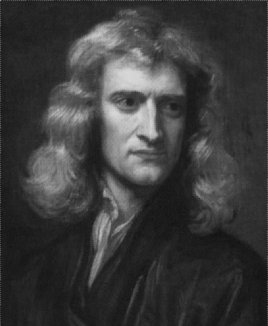
\includegraphics[width=\textwidth]{figures/Newton}
  \end{textblock}
  \begin{itemize}
  \item Standard form of a nonlinear system
    \[ F(u) = 0 \]
  \item Iteration
    \begin{align*}
      \text{Solve:} & \qquad J(u) w = -F(u) \\
      \text{Update:} & \qquad u^+ \gets u + w
    \end{align*}
    \item Quadratically convergent near a root: $\abs{u^{n+1}-u^*} \in \bigO\Big(\abs{u^n-u^*}^2\Big)$
    \item Picard is the same operation with a different $J(u)$
  \end{itemize}
  \begin{example}[Nonlinear Poisson]
    \begin{align*}
      F(u)=0 \quad &\sim\quad -\div\big[ (1+u^2) \grad u \big] - f = 0 \\
      J(u)w \quad &\sim\quad  -\div\big[(1+u^2)\grad w + 2uw\grad u \Big]
    \end{align*}
  \end{example}
  % \begin{example}[$\pp$-Bratu]
  %   Suppose $F$ is a discretization of
  %   \[ -\nabla \cdot \big( \eta \nabla u \big) - \lambda e^u - f = 0 \]
  %   \[\eta(\gamma) = (\epsilon^2+\gamma)^{\frac{\pfrak-2}{2}}, \qquad\quad \gamma = \half \abs{\nabla u}^2. \]
  %   Then $J(u)w$ is a discretization of
  %   \[ -\nabla \cdot \big( \eta \nabla w + \eta' (\nabla u \cdot \nabla w)\nabla u \big) - \lambda e^{u} w . \]
  % \end{example}
\end{frame}

\subsection{Linear Algebra background/theory}
\begin{frame}{Matrices}
  \begin{definition}<1->[Matrix]
    A \alert{matrix} is a linear transformation between finite dimensional vector spaces.
  \end{definition}
  \begin{definition}<2->[Forming a matrix]
    \alert{Forming} or \alert{assembling} a matrix means defining it's action in terms of entries (usually stored in a sparse format).
  \end{definition}
\end{frame}

\begin{frame}{Important matrices}
  \begin{enumerate}
  \item Sparse (e.g.~discretization of a PDE operator)
  \item \alert<2,4>{Inverse of \emph{anything} interesting $B = A^{-1}$}
  \item \alert<4>{Jacobian of a nonlinear function $J y = \lim_{\epsilon \to 0} \frac{F(x + \epsilon y) - F(x)}{\epsilon}$}
  \item \alert<2,4>{Fourier transform $\mathcal{F},\mathcal{F}^{-1}$}
  \item \alert<2,4>{Other fast transforms, e.g. Fast Multipole Method}
  \item \alert<2,4>{Low rank correction $B = A + u v^T$}
  \item \alert<2,4>{Schur complement $S = D - C A^{-1} B$}
  \item \alert<3,4>{Tensor product $A = \sum_e A_x^e \otimes A_y^e \otimes A_z^e$}
  \item \alert<3,4>{Linearization of a few steps of an explicit integrator}
  \end{enumerate}
  \begin{columns}\begin{column}{0.3\textwidth}\end{column}\begin{column}{0.7\textwidth}
  \begin{itemize}
  \item<only@2> These matrices are \alert<2>{dense}.  Never form them.
  \item<only@3>{Thes are \alert<3>{not very sparse}.}
    Don't form them.
  \item<only@4> {None of these matrices ``have entries''}
  \end{itemize}
\end{column}
\end{columns}
\end{frame}

\begin{frame}{What can we do with a matrix that doesn't have entries?}
  \begin{block}{Krylov solvers for $A x = b$}
    \begin{itemize}
    \item Krylov subspace: $\{b, Ab, A^2b, A^3b, \dotsc\}$
    \item Convergence rate depends on the spectral properties of the matrix
      \begin{itemize}
      \item Existance of small polynomials $p_n(A) < \epsilon$ where $p_n(0) = 1$.
      \item condition number $\kappa(A) = \norm{A} \norm{A^{-1}} = \sigma_{\text{max}}/\sigma_{\text{min}}$
      \item distribution of singular values, spectrum $\Lambda$, pseudospectrum $\Lambda_\epsilon$
%      \item $\epsilon$-pseudospectrum $\Lambda_\epsilon$, spectrum of $A + E$ where $\norm{E} < \epsilon$
      \end{itemize}
    \item For any popular Krylov method $\mathcal{K}$, there is a matrix
      of size $m$, such that $\mathcal{K}$ outperforms all other methods
      by a factor at least $\bigO(\sqrt{m})$~[Nachtigal et. al., 1992]%\cite{nachtigal1992fnm}
    \end{itemize}
  \end{block}
  \begin{block}{Typically...}
    \begin{itemize}
    \item The action $y \gets A x$ can be computed in $\bigO(m)$
    \item Aside from matrix multiply, the $n^{\text{th}}$ iteration requires at most $\bigO(mn)$
    \end{itemize}
  \end{block}
\end{frame}

\begin{frame}{GMRES}
  Brute force minimization of residual in $\{b,Ab,A^2b,\dotsc\}$
  \begin{enumerate}
  \item Use Arnoldi to orthogonalize the $n$th subspace, producing
    \[ A Q_n = Q_{n+1} H_n \]
  \item Minimize residual in this space by solving the overdetermined system
    \[ H_n y_n = e_1^{(n+1)} \]
    using $QR$-decomposition, updated cheaply at each iteration.
  \end{enumerate}
  Properties
  \begin{itemize}
  \item Converges in $n$ steps for all right hand sides if there exists a polynomial of degree $n$
    such that $\norm{p_n(A)} < \textit{tol}$ and $p_n(0)=1$.
  \item Residual is monotonically decreasing, robust in practice
  \item Restarted variants are used to bound memory requirements
  \end{itemize}
\end{frame}


% \section{$\pfrak$-Bratu}
\begin{frame}{The $\pfrak$-Bratu equation}
  \begin{itemize}
  \item 2-dimensional model problem
    \begin{equation*}
      -\div \big(\abs{\nabla u}^{\pfrak-2} \nabla u \big) - \lambda e^u - f = 0, \qquad 1 \le \pfrak \le \infty, \quad \lambda < \lambda_{\text{crit}}(\pfrak)
    \end{equation*}
    Singular or degenerate when $\nabla u = 0$, turning point at $\lambda_{\text{crit}}$.
  \item Regularized variant
    \begin{gather*}
      -\div (\eta \grad u) - \lambda e^u - f = 0 \\
      \eta(\gamma) = (\epsilon^2 + \gamma)^{\frac{\pfrak-2}{2}} \qquad \gamma(u) = \half \abs{\grad u}^2
    \end{gather*}
  \item Jacobian
    \begin{gather*}
      J(u) w \sim -\div \big[ (\eta \bm 1 + \eta' \nabla u \otimes \nabla u) \grad w \big] - \lambda e^u w \\
      \eta' = \frac{\pfrak-2}{2} \eta / (\epsilon^2 + \gamma)
    \end{gather*}
    Physical interpretation: conductivity tensor flattened in direction $\grad u$ %($\pfrak < 2$)
  \end{itemize}
\end{frame}

% \frame{
%   \begin{itemize}
%   \item Start with 2-Laplacian plus Bratu, define only residuals
%   \item Matrix-free Jacobians, no preconditioning \code{-snes\_mf}
%   \item \shell{hg update -r\Rsnesmf}
%   \item \shell{./pbratu -da\_grid\_x 10 -da\_grid\_y 10 -snes\_mf -snes\_monitor -ksp\_converged\_reason}
%   \item \shell{./pbratu -da\_grid\_x 20 -da\_grid\_y 20 -snes\_mf -snes\_monitor -ksp\_converged\_reason}
%   \item \shell{./pbratu -da\_grid\_x 40 -da\_grid\_y 40 -snes\_mf -snes\_monitor -ksp\_converged\_reason}
%   \end{itemize}
% }

\subsection{Nonlinear solvers: SNES}
\frame{
\frametitle{Flow Control for a PETSc Application}

\begin{center}
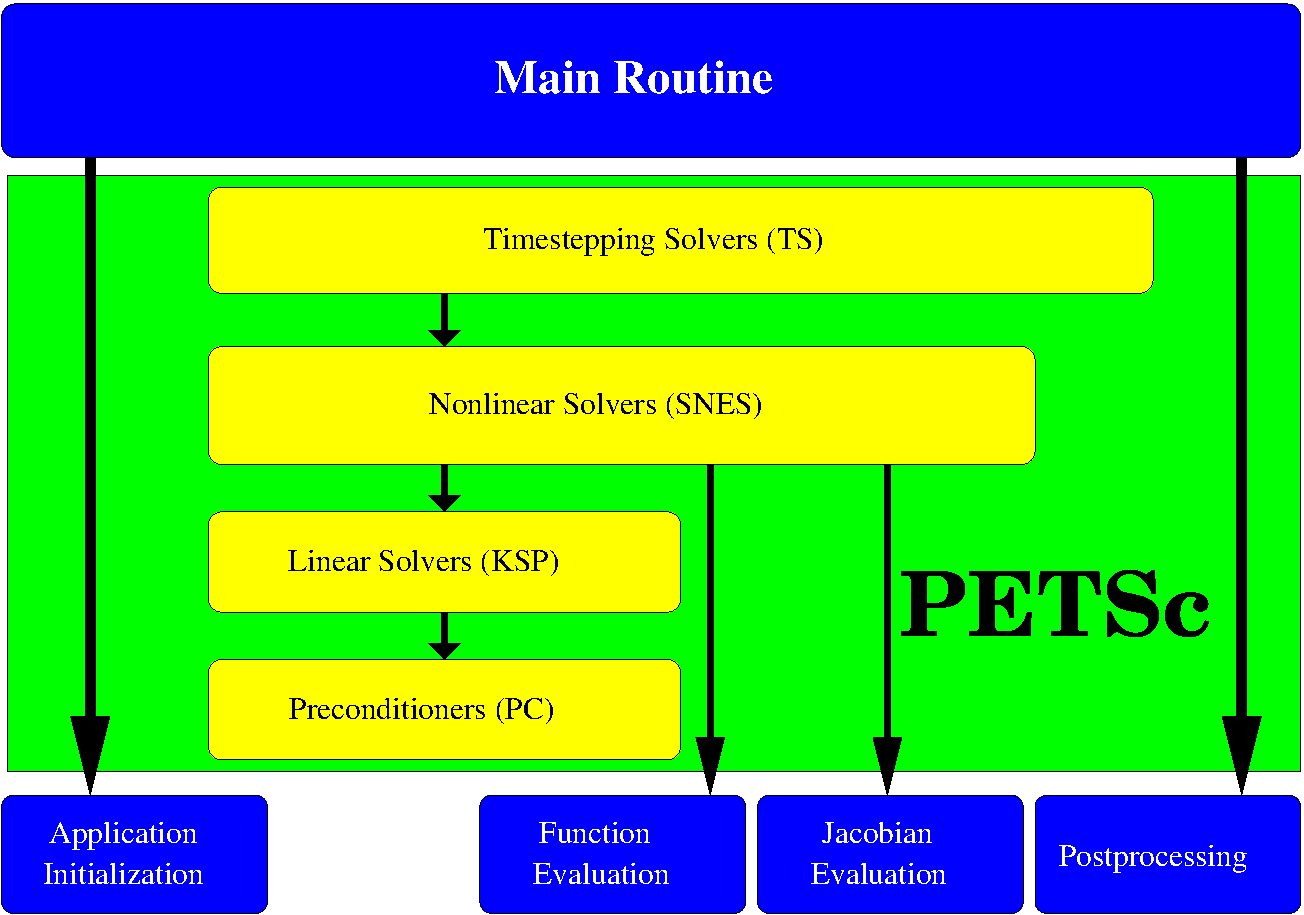
\includegraphics[width=4.0in]{figures/SNES/FlowControl}
\end{center}
}

\begin{frame}
\frametitle{SNES Paradigm}

The SNES interface is based upon callback functions
\begin{itemize}
  \item \code{FormFunction()}, set by \code{SNESSetFunction()}

  \medskip

  \item \code{FormJacobian()}, set by \code{SNESSetJacobian()}
\end{itemize}

\bigskip

  When PETSc needs to evaluate the nonlinear residual $F(x)$,
\begin{itemize}
  \item Solver calls the {\bf user's} function

  \medskip

  \item User function gets application state through the {\kb ctx} variable
  \begin{itemize}
    \item PETSc \emph{never} sees application data
  \end{itemize}
\end{itemize}
\end{frame}

\begin{frame}{SNES Function}

The user provided function which calculates the nonlinear residual has signature
\begin{center}
  {\small \mint{c}|PetscErrorCode (*func)(SNES snes,Vec x,Vec r,void *ctx)|}
\end{center}
\begin{itemize}
  \item[{\kb x}:] The current solution
  \item[{\kb r}:] The residual
  \item[{\kb ctx}:] The user context passed to {\kb SNESSetFunction()}
  \begin{itemize}
    \item Use this to pass application information, e.g. physical constants
  \end{itemize}
\end{itemize}

\end{frame}

\begin{frame}[fragile]{SNES Jacobian}
The user provided function which calculates the Jacobian has signature
\begin{minted}{c}
PetscErrorCode (*func)(SNES snes,Vec x,Mat *J,Mat *M,
                       MatStructure *flag,void *ctx)
\end{minted}

\begin{itemize}
  \item[{\kb x}:] The current solution
  \item[{\kb J}:] The Jacobian
  \item[{\kb M}:] The Jacobian preconditioning matrix (possibly J itself)
  \item[{\kb ctx}:] The user context passed to {\kb SNESSetFunction()}
  \begin{itemize}
    \item Use this to pass application information, e.g. physical constants
  \end{itemize}

  \item Possible {\kb MatStructure} values are:
  \begin{itemize}
    \item SAME\_NONZERO\_PATTERN
    \item DIFFERENT\_NONZERO\_PATTERN
  \end{itemize}
\end{itemize}

Alternatively, you can use
\begin{itemize}
  \item a builtin sparse finite difference approximation (``coloring'')
  \item automatic differentiation (ADIC/ADIFOR)
\end{itemize}

\end{frame}


\subsection{Structured grid distribution: DA}
\begin{frame}{Distributed Array}
  \begin{itemize}
  \item Interface for topologically structured grids
  \item Defines (topological part of) a finite-dimensional function space
    \oneitem{Get an element from this space: \code{DACreateGlobalVector()}}
  \item Provides parallel layout
  \item Refinement and coarsening
    \oneitem{\code{DARefineHierarchy()}}
  \item Ghost value coherence
    \oneitem{\code{DAGlobalToLocalBegin()}}
  \item Matrix preallocation: \oneitem{\code{DAGetMatrix()}}
  \end{itemize}
\end{frame}
\frame{
\frametitle{Ghost Values}

To evaluate a local function $f(x)$, each process requires
\begin{itemize}
  \item its local portion of the vector $x$
  \item its \cyan{ghost values}, bordering portions of $x$ owned by neighboring processes
\end{itemize}

\begin{center}
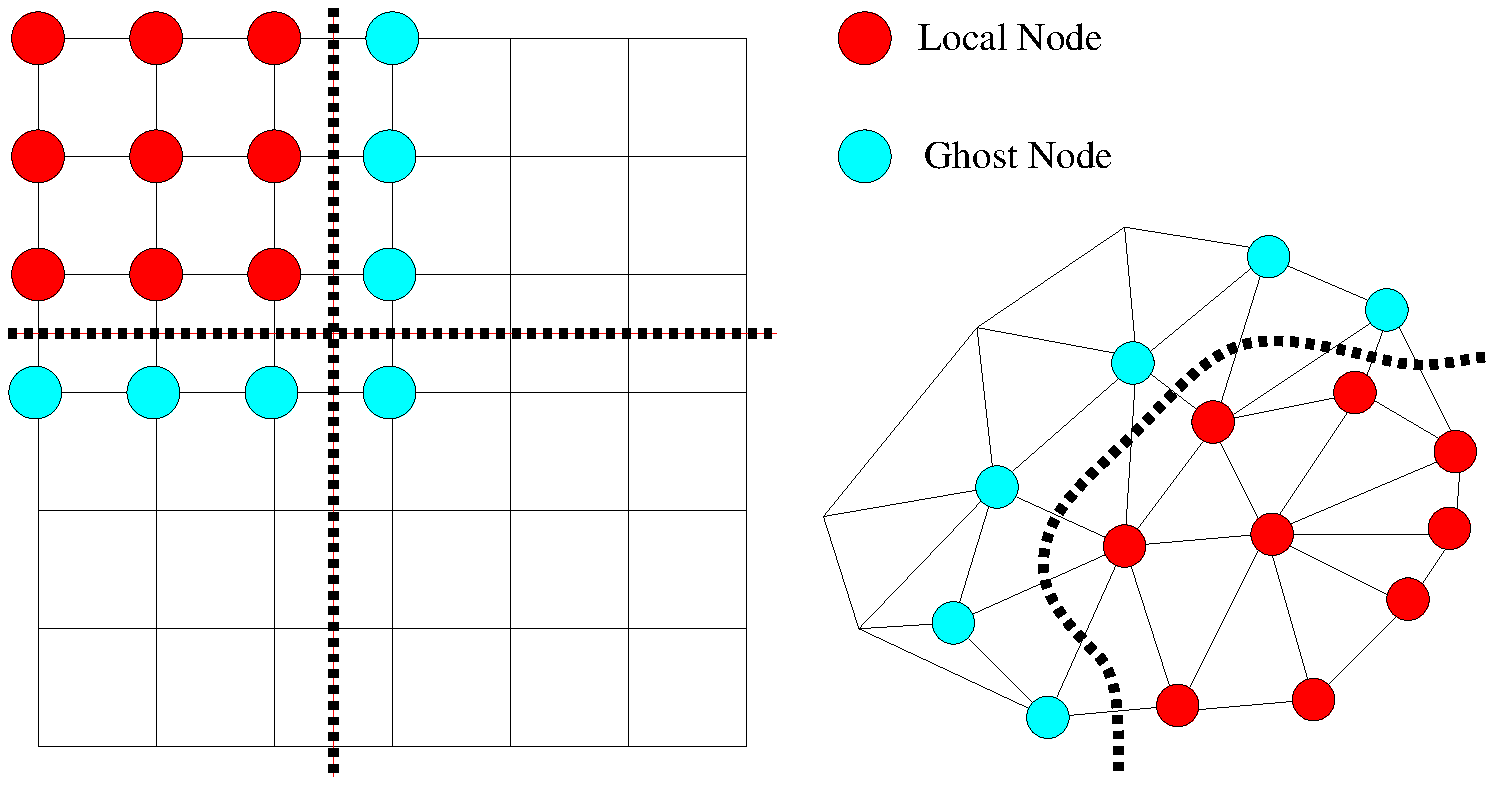
\includegraphics[width=4in]{figures/DA/GhostValues}
\end{center}
}

\begin{frame}{DA Global Numberings}

\begin{center}
\begin{tabular}{cc}
\begin{tabular}{c}
\begin{tabular}{|ccc|cc|}
\hline
\multicolumn{3}{|c|}{Proc 2} & \multicolumn{2}{c|}{Proc 3} \\
\hline
25 & 26 & 27 & 28 & 29 \\
20 & 21 & 22 & 23 & 24 \\
15 & 16 & 17 & 18 & 19 \\
\hline
10 & 11 & 12 & 13 & 14 \\
 5 &  6 &  7 &  8 &  9 \\
 0 &  1 &  2 &  3 &  4 \\
\hline
\multicolumn{3}{|c|}{Proc 0} & \multicolumn{2}{c|}{Proc 1} \\
\hline
\end{tabular} \\
Natural numbering
\end{tabular}
& 
\begin{tabular}{c}
\begin{tabular}{|ccc|cc|}
\hline
\multicolumn{3}{|c|}{Proc 2} & \multicolumn{2}{c|}{Proc 3} \\
\hline
21 & 22 & 23 & 28 & 29 \\
18 & 19 & 20 & 26 & 27 \\
15 & 16 & 17 & 24 & 25 \\
\hline
 6 &  7 &  8 & 13 & 14 \\
 3 &  4 &  5 & 11 & 12 \\
 0 &  1 &  2 &  9 & 10 \\
\hline
\multicolumn{3}{|c|}{Proc 0} & \multicolumn{2}{c|}{Proc 1} \\
\hline
\end{tabular}\\
PETSc numbering
\end{tabular}
\end{tabular}
\end{center}
\end{frame}

\begin{frame}{DMDA Global vs. Local Numbering}

\begin{itemize}
  \item {\bf Global}: Each vertex has a unique id belongs on a unique process

  \item {\bf Local}: Numbering includes vertices from neighboring processes
  \begin{itemize}
    \item These are called \cyan{ghost} vertices
  \end{itemize}
\end{itemize}

\begin{center}
\begin{tabular}{cc}
\begin{tabular}{c}
\begin{tabular}{|ccc|cc|}
\hline
\multicolumn{3}{|c|}{Proc 2} & \multicolumn{2}{c|}{Proc 3} \\
\hline
 X &  X &  X &  X &  X \\
 X &  X &  X &  X &  X \\
\cyan{12} & \cyan{13} & \cyan{14} & \cyan{15} &  X \\
\hline
 8 &  9 & 10 & \cyan{11} &  X \\
 4 &  5 &  6 &  \cyan{7} &  X \\
 0 &  1 &  2 &  \cyan{3} &  X \\
\hline
\multicolumn{3}{|c|}{Proc 0} & \multicolumn{2}{c|}{Proc 1} \\
\hline
\end{tabular} \\
Local numbering
\end{tabular}
& 
\begin{tabular}{c}
\begin{tabular}{|ccc|cc|}
\hline
\multicolumn{3}{|c|}{Proc 2} & \multicolumn{2}{c|}{Proc 3} \\
\hline
21 & 22 & 23 & 28 & 29 \\
18 & 19 & 20 & 26 & 27 \\
15 & 16 & 17 & 24 & 25 \\
\hline
 6 &  7 &  8 & 13 & 14 \\
 3 &  4 &  5 & 11 & 12 \\
 0 &  1 &  2 &  9 & 10 \\
\hline
\multicolumn{3}{|c|}{Proc 0} & \multicolumn{2}{c|}{Proc 1} \\
\hline
\end{tabular}\\
Global numbering
\end{tabular}
\end{tabular}
\end{center}
\end{frame}

\frame{
\frametitle{DM Vectors}

\begin{itemize}
  \item The DM object contains only layout (topology) information
  \begin{itemize}
    \item All field data is contained in PETSc {\kb Vec}s
  \end{itemize}

  \item Global vectors are parallel 
  \begin{itemize}
    \item Each process stores a unique local portion
    \item {\kb DMCreateGlobalVector(DM dm, Vec *gvec)}
  \end{itemize}

  \item Local vectors are sequential (and usually temporary)
  \begin{itemize}
    \item Each process stores its local portion plus ghost values
    \item {\kb DMCreateLocalVector(DM dm, Vec *lvec)}
    \item includes ghost values!
  \end{itemize}

  \item Coordinate vectors store the mesh geometry
    \begin{itemize}
    \item \code{DMDAGetCoordinates(DM dm, Vec *coords)}
    \item Can be manipulated with their own DMDA \\
      \code{DMDAGetCoordinateDA(DM dm,DM *cda)}
    \end{itemize}
\end{itemize}
}

\begin{frame}{Updating Ghosts}

Two-step process enables overlapping\\
computation and communication

\medskip

\begin{itemize}
  \item {\kb DMGlobalToLocalBegin(dm, gvec, mode, lvec)}
  \begin{itemize}
    \item {\kb gvec} provides the data 
    \item {\kb mode} is either {\kb INSERT\_VALUES} or {\kb ADD\_VALUES}
    \item {\kb lvec} holds the local and ghost values
  \end{itemize}

  \item {\kb DMGlobalToLocalEnd(dm, gvec, mode, lvec)}
  \begin{itemize}
    \item Finishes the communication
  \end{itemize}
\end{itemize}

\medskip

The process can be reversed with {\kb DMLocalToGlobalBegin()} and {\kb DMLocalToGlobalEnd()}.
\end{frame}

\frame{
\frametitle{DMDA Stencils}

Both the \blue{box} stencil and \blue{star} stencil are available.

\begin{center}
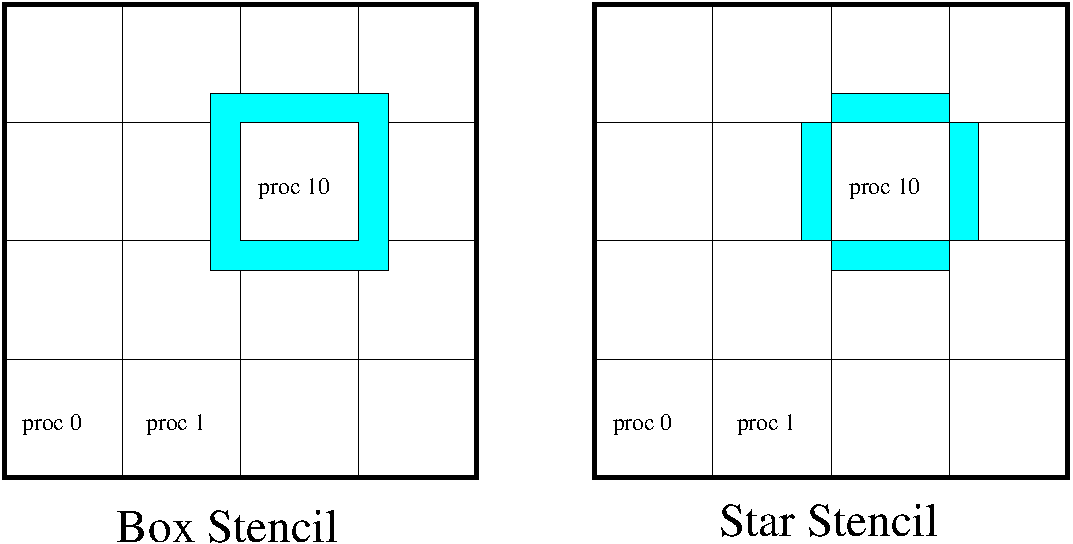
\includegraphics[width=4.5in]{figures/DA/Stencils}
\end{center}
}

\frame{
\frametitle{Creating a DMDA}

{\small \kb DMDACreate2d(comm, xbdy, ybdy, type, M, N, m, n, \\
\qquad\qquad\qquad  dof, s, lm[], ln[], DA *da)}
\begin{columns}\begin{column}{0.15\textwidth}\end{column}\begin{column}{0.85\textwidth}
  \begin{itemize}
  \item[{\kb xbdy,ybdy}:] Specifies periodicity or ghost cells
  \begin{itemize}
    \item {\kb DMDA\_BOUNDARY\_NONE}, {\kb DMDA\_BOUNDARY\_GHOSTED}, {\kb DMDA\_BOUNDARY\_MIRROR}, {\kb DMDA\_BOUNDARY\_PERIODIC}
  \end{itemize}
  \item[{\kb type}:] Specifies stencil
  \begin{itemize}
    \item {\kb DMDA\_STENCIL\_BOX} or {\kb DMDA\_STENCIL\_STAR}
  \end{itemize}
  \item[{\kb M,N}:] Number of grid points in x/y-direction
  \item[{\kb m,n}:] Number of processes in x/y-direction
  \item[{\kb dof}:] Degrees of freedom per node
  \item[{\kb s}:] The stencil width
  \item[{\kb lm,ln}:] Alternative array of local sizes
  \begin{itemize}
    \item Use {\kb PETSC\_NULL} for the default
  \end{itemize}
\end{itemize}
\end{column} \end{columns}
}

\begin{frame}{Working with the local form}
  Wouldn't it be nice if we could just write our code for the natural numbering?
  \begin{itemize}
  \item Yes, that's what \code{DMDAVecGetArray()} is for.
  \item Also, DMDA offers \emph{local} callback functions
    \begin{itemize}
    \item \code{FormFunctionLocal()}, set by \code{DMDASetLocalFunction()}
      
      \medskip
      
    \item \code{FormJacobianLocal()}, set by \code{DMDASetLocalJacobian()}
    \end{itemize}

    \bigskip

  \item When PETSc needs to evaluate the nonlinear residual $F(x)$,
    \begin{itemize}
    \item Each process evaluates the local residual

      \medskip

    \item PETSc assembles the global residual automatically
      \begin{itemize}
      \item Uses \code{DMLocalToGlobal()} method
      \end{itemize}
    \end{itemize}
  \end{itemize}
\end{frame}

\frame{
\frametitle{DA Local Function}

The user provided function which calculates the nonlinear residual in 2D has signature \\
{\kb PetscErrorCode (*lfunc)(DALocalInfo *info, \\
  \qquad \qquad \qquad Field **x, Field **r, void *ctx)}
\begin{columns}\begin{column}{0.15\textwidth}\end{column}\begin{column}{0.85\textwidth}
\begin{itemize}
  \item[{\kb info}:] All layout and numbering information
  \item[{\kb x}:] The current solution
  \begin{itemize}
    \item Notice that it is a multidimensional array
  \end{itemize}
  \item[ {\kb r}:] The residual
  \item[ {\kb ctx}:] The user context passed to {\kb DASetLocalFunction()}
\end{itemize}
\end{column}\end{columns}

\bigskip

The local DA function is activated by calling
\begin{center}
  {\kb SNESSetFunction(snes, r, SNESDAFormFunction, ctx)}
\end{center}
}

\begin{frame}[fragile]
\frametitle{Bratu Residual Evaluation}

\begin{equation*}
  -\Delta u - \lambda e^{u} = 0
\end{equation*}

\small
\begin{minted}[fontsize=\footnotesize]{c}
BratuResidualLocal(DMDALocalInfo *info,Field **x,Field **f,
                   UserCtx *user)
{
  /* Not Shown: Handle boundaries */
  /* Compute over the interior points */
  for(j = info->ys; j < info->ys+info->ym; j++) {
    for(i = info->xs; i < info->xs+info->xm; i++) {
      u       = x[j][i];
      u_xx    = (2.0*u - x[j][i-1] - x[j][i+1])*hydhx;
      u_yy    = (2.0*u - x[j-1][i] - x[j+1][i])*hxdhy;
      f[j][i] = u_xx + u_yy - hx*hy*lambda*exp(u);
    }
  }
}
\end{minted}

\begin{center}\small
\$PETSC\_DIR/src/snes/examples/tutorials/ex5.c
\end{center}
\end{frame}


\begin{frame}{Start with 2-Laplacian plus Bratu nonlinearity}
  \begin{itemize}
  \item Matrix-free Jacobians, no preconditioning \code{-snes\_mf}
  \item \shell{hg update -r\Rsnesmflambda}
  \item \shell{./pbratu -da\_grid\_x 10 -da\_grid\_y 10 \\ -lambda 6.7 -snes\_mf -snes\_monitor -ksp\_converged\_reason}
  \item \shell{./pbratu -da\_grid\_x 20 -da\_grid\_y 20 \\ -lambda 6.7 -snes\_mf -snes\_monitor -ksp\_converged\_reason}
  \item \shell{./pbratu -da\_grid\_x 40 -da\_grid\_y 40 \\ -lambda 6.7 -snes\_mf -snes\_monitor -ksp\_converged\_reason}
  \item Watch linear and nonlinear convergence
  \end{itemize}
\end{frame}

\begin{frame}{Add $\pfrak$ nonlinearity}
  \begin{itemize}
  \item Matrix-free Jacobians, no preconditioning \code{-snes\_mf}
  \item \shell{hg update -r\Rsnesmfp}
  \item \shell{./pbratu -da\_grid\_x 10 -da\_grid\_y 10 \\ -lambda 1 -p 1.3 -snes\_mf -snes\_monitor -ksp\_converged\_reason}
  \item \shell{./pbratu -da\_grid\_x 20 -da\_grid\_y 20 \\ -lambda 1 -p 1.3 -snes\_mf -snes\_monitor -ksp\_converged\_reason}
  \item \shell{./pbratu -da\_grid\_x 40 -da\_grid\_y 40 \\ -lambda 1 -p 1.3 -snes\_mf -snes\_monitor -ksp\_converged\_reason}
  \item Watch linear and nonlinear convergence
  \end{itemize}
\end{frame}

\subsection{Preconditioning}
\begin{frame}{Preconditioning}
  \begin{block}{Idea: improve the conditioning of the Krylov operator}
    \begin{itemize}
    \item Left preconditioning
      \vspace{-1em}
      \begin{gather*}
        (P^{-1} A) x = P^{-1} b \\
        \{ P^{-1} b, (P^{-1}A) P^{-1} b, (P^{-1}A)^2 P^{-1} b, \dotsc \}
      \end{gather*}
    \item Right preconditioning
      \vspace{-1em}
      \begin{gather*}
        (A P^{-1}) P x = b \\
        \{ b, (P^{-1}A)b, (P^{-1}A)^2b, \dotsc \}
      \end{gather*}
    \item The product $P^{-1}A$ or $A P^{-1}$ is \emph{not} formed.
    \end{itemize}
  \end{block}
  \begin{definition}[Preconditioner]
      A \emph{preconditioner} $\PP$ is a method for constructing a
matrix (just a linear function, not assembled!)  $P^{-1} = \PP(A,A_p)$
using a matrix $A$ and extra information $A_p$, such that the spectrum
of $P^{-1}A$ (or $A P^{-1}$) is well-behaved.
    \end{definition}
\end{frame}

\begin{frame}{Preconditioning}
  \begin{definition}[Preconditioner]
      A \emph{preconditioner} $\PP$ is a method for constructing a matrix
      $P^{-1} = \PP(A,A_p)$ using a matrix $A$ and extra information $A_p$, such that
      the spectrum of $P^{-1}A$ (or $A P^{-1}$) is well-behaved.
    \end{definition}
    \begin{itemize}
    \item $P^{-1}$ is dense, $P$ is often not available and is not needed
    \item $A$ is rarely used by $\PP$, but $A_p = A$ is common
    \item $A_p$ is often a sparse matrix, the ``preconditioning matrix''
    \item Matrix-based: Jacobi, Gauss-Seidel, SOR, ILU(k), LU
    \item Parallel: Block-Jacobi, Schwarz, Multigrid, FETI-DP, BDDC
    \item Indefinite: Schur-complement, Domain Decomposition, Multigrid
    \end{itemize}
\end{frame}


\begin{frame}{Questions to ask when you see a matrix}
  \begin{enumerate}
  \item What do you want to do with it?
    \begin{itemize}
    \item Multiply with a vector
    \item Solve linear systems or eigen-problems
    \end{itemize}
  \item How is the conditioning/spectrum?
    \begin{itemize}
    \item distinct/clustered eigen/singular values?
    \item symmetric positive definite ($\sigma(A) \subset \R^+$)?
    \item nonsymmetric definite ($\sigma(A) \subset \{z \in \C : \Re [z] > 0 \}$)?
    \item indefinite?
    \end{itemize}
  \item How dense is it?
    \begin{itemize}
    \item block/banded diagonal?
    \item sparse unstructured?
    \item denser than we'd like?
    \end{itemize}
  \item Is there a better way to compute $Ax$?
  \item Is there a different matrix with similar spectrum, but nicer properties?
  \item \alert<2>{How can we precondition $A$?}
  \end{enumerate}
\end{frame}

\begin{frame}{Relaxation}
  Split into lower, diagonal, upper parts: \alert{$ A = L + D + U $}
  \begin{block}{Jacobi}
    Cheapest preconditioner: $P^{-1} = D^{-1}$
  \end{block}
  \begin{block}{Successive over-relaxation (SOR)}
    \begin{gather*}
      \left(L + \frac 1 \omega D\right) x_{n+1} = \left[\left(\frac
          1\omega-1\right)D - U\right] x_n + \omega b \\
      P^{-1} = \text{$k$ iterations starting with $x_0=0$}
    \end{gather*}
    \begin{itemize}
    \item Implemented as a sweep
    \item $\omega = 1$ corresponds to Gauss-Seidel
    \item Very effective at removing high-frequency components of residual
    \end{itemize}
  \end{block}
\end{frame}

\begin{frame}[shrink=5]{Factorization}
  Two phases
  \begin{itemize}
  \item symbolic factorization: find where fill occurs, only uses sparsity pattern
  \item numeric factorization: compute factors
  \end{itemize}
  \begin{block}{LU decomposition}
    \begin{itemize}
    \item Ultimate preconditioner
    \item Expensive, for $m\times m$ sparse matrix with bandwidth $b$, traditionally requires $\bigO(mb^2)$ time and $\bigO(mb)$ space.
      \begin{itemize}
      \item Bandwidth scales as $m^{\frac{d-1}{d}}$ in $d$-dimensions
      \item Optimal in 2D: $\bigO(m \cdot \log m)$ space, $\bigO(m^{3/2})$ time
      \item Optimal in 3D: $\bigO(m^{4/3})$ space, $\bigO(m^2)$ time
      \end{itemize}
    \item Symbolic factorization is problematic in parallel
    \end{itemize}
  \end{block}
  \begin{block}{Incomplete LU}
    \begin{itemize}
    \item Allow a limited number of levels of fill:
      ILU($k$)
    \item Only allow fill for entries that exceed threshold: ILUT
    \item Very poor scaling in parallel, don't bother beyond 8 PEs.
    \item No guarantees
    \end{itemize}
  \end{block}
\end{frame}

\begin{frame}{1-level Domain decomposition}
  Domain size $L$, subdomain size $H$, element size $h$
  \begin{block}{Overlapping/Schwarz}
    \begin{itemize}\item Solve Dirichlet problems on overlapping
      subdomains
    \item No overlap: $\textit{its} \in \bigO\big( \frac{L}{\sqrt{Hh}} \big)$
    \item Overlap $\delta$: $\textit{its} \in \big( \frac L {\sqrt{H\delta}} \big)$
    \end{itemize}
  \end{block}
  \begin{block}{Neumann-Neumann}
    \begin{itemize}
    \item Solve Neumann problems on non-overlapping subdomains
    \item $\textit{its} \in \bigO\big( \frac{L}{H}(1+\log\frac H h) \big)$
    \item Tricky null space issues (floating subdomains)
    \item Need subdomain matrices, net globally assembled matrix.
    \end{itemize}
  \end{block}
  \begin{itemize}
  \item Multilevel variants knock off the leading $\frac L H$
  \item Both overlapping and nonoverlapping with this bound
  \end{itemize}
  % \begin{block}{BDDC and FETI-DP}
  %   \begin{itemize}
  %   \item Neumann problems on subdomains with
  %     coarse grid correction
  %   \item $\textit{its} \in \bigO\big(1 + \log\frac H h \big)$
  %   \end{itemize}
  %   \includegraphics[width=0.7\textwidth]{bddc}
  % \end{block}
\end{frame}

\begin{frame}[shrink=5]{Multigrid}
  \begin{block}{Hierarchy: Interpolation and restriction operators}
    \begin{equation*}
    \II^\uparrow : X_{\text{coarse}} \to X_{\text{fine}} \qquad
    \II^\downarrow :  X_{\text{fine}} \to X_{\text{coarse}}
  \end{equation*}
  \end{block}
  \begin{itemize}
  \item Geometric: define problem on multiple levels, use grid to compute hierarchy
  \item Algebraic: define problem only on finest level, use matrix structure to build hierarchy
  \end{itemize}
  \begin{block}{Galerkin approximation}
    Assemble this matrix: $A_{\text{coarse}} = \II^\downarrow A_{\text{fine}} \II^\uparrow$
  \end{block}
  \begin{block}{Application of multigrid preconditioner ($V$-cycle)}
    \begin{itemize}
    \item Apply pre-smoother on fine level (any preconditioner)
    \item Restrict residual to coarse level with $\II^\downarrow$
    \item Solve on coarse level $A_{\text{coarse}} x = r$
    \item Interpolate result back to fine level with $\II^\uparrow$
    \item Apply post-smoother on fine level (any preconditioner)
    \end{itemize}
  \end{block}
\end{frame}

\begin{frame}{Multigrid convergence properties}
  \begin{itemize}
  \item Textbook: $P^{-1}A$ is spectrally equivalent to identity
    \begin{itemize}
    \item Constant number of iterations to converge up to discretization error
    \end{itemize}
  \item Most theory applies to SPD systems
    \begin{itemize}
    \item variable coefficients (\eg discontinuous): low energy interpolants
    \item mesh- and/or physics-induced anisotropy: semi-coarsening/line smoothers
    \item complex geometry: difficult to have meaningful coarse levels
    \end{itemize}
  \item Deeper algorithmic difficulties
    \begin{itemize}
    \item nonsymmetric (\eg advection, shallow water, Euler) \\
    \item indefinite (\eg incompressible flow, Helmholtz)
    \end{itemize}
  \item Performance considerations
    \begin{itemize}
    \item Aggressive coarsening is critical in parallel
    \item Most theory uses SOR smoothers, ILU often more robust
    \item Coarsest level usually solved semi-redundantly with direct solver
    \end{itemize}
  \item Multilevel Schwarz is essentially the same with different language
    \begin{itemize}
    \item assume strong smoothers, emphasize aggressive coarsening
    \end{itemize}
  \end{itemize}
\end{frame}


\begin{frame}{Finite Difference Jacobians}
  PETSc can compute and explicitly store a Jacobian via 1st-order FD
  \begin{itemize}
  \item Dense
    \begin{itemize}
    \item Activated by {\kb -snes\_fd}
    \item Computed by {\kb SNESDefaultComputeJacobian()}
    \end{itemize}
  \item Sparse via colorings
    \begin{itemize}
    \item Coloring is created by {\kb MatFDColoringCreate()}
    \item Computed by {\kb SNESDefaultComputeJacobianColor()}
    \end{itemize}
  \end{itemize}
  Can also use Matrix-free Newton-Krylov via 1st-order FD
  \begin{itemize}
  \item Activated by {\kb -snes\_mf} without preconditioning
  \item Activated by {\kb -snes\_mf\_operator} with user-defined preconditioning
    \begin{itemize}
    \item Uses preconditioning matrix from {\kb SNESSetJacobian()}
    \end{itemize}
  \end{itemize}
\end{frame}


\begin{frame}{Add finite difference Jacobian by coloring}
  \begin{itemize}
  \item \shell{hg update -r\Rcolor}
  \item \shell{./pbratu -da\_grid\_x 10 -da\_grid\_y 10 \\ -lambda 1 -p 1.3 -snes\_fd -snes\_monitor -ksp\_converged\_reason}
  \item \shell{./pbratu -da\_grid\_x 10 -da\_grid\_y 10 \\ -lambda 1 -p 1.3 -fd\_jacobian -snes\_monitor -ksp\_converged\_reason}
  \item \shell{./pbratu -da\_grid\_x 10 -da\_grid\_y 10 \\ -lambda 1 -p 1.3 -fd\_jacobian -snes\_monitor -ksp\_converged\_reason}
  \item Try some different preconditioners (\code{jacobi,sor,asm,hypre,ml})
  \item Try changing the physical parameters
  \item May need \code{-mat\_fd\_type ds}
  \end{itemize}
\end{frame}

\subsection{Matrix Redux}
\begin{frame}{Matrices, redux}
What are PETSc matrices?
\begin{itemize}
\item Linear operators on finite dimensional vector spaces. (snarky)
  \item<2> Fundamental objects for storing stiffness matrices and Jacobians
  \item<2> Each process locally owns a contiguous set of rows
  \item<2> Supports many data types
  \begin{itemize}
    \item AIJ, Block AIJ, Symmetric AIJ, Block Diagonal, etc.
  \end{itemize}
  \item<2> Supports structures for many packages
  \begin{itemize}
    \item MUMPS, Spooles, SuperLU, UMFPack, DSCPack
  \end{itemize}
\end{itemize}
\end{frame}

\begin{frame}{How do I create matrices?}

\begin{itemize}
  \item {\kb MatCreate(MPI\_Comm, Mat *)}
  \item {\kb MatSetSizes(Mat, int m, int n, int M, int N)}
  \item {\kb MatSetType(Mat, MatType typeName)}
  \item {\kb MatSetFromOptions(Mat)}
  \begin{itemize}
    \item Can set the type at runtime
  \end{itemize}
  \item {\kb MatMPIBAIJSetPreallocation(Mat,...)} %(Mat,int bs,int d_nz,const int
                                %d_nnz[],int o_nz,const int o_nnz[])}
    \oneitem{important for assembly performance, more tomorrow}
  \item {\kb MatSetBlockSize(Mat, int bs)}
    \oneitem{for vector problems}
  \item {\kb MatSetValues(Mat,...)}
  \begin{itemize}
    \item {\bf MUST} be used, but does automatic communication
  \end{itemize}
\end{itemize}

\end{frame}

\begin{frame}{Matrix Polymorphism}

The PETSc {\kb Mat} has a single user interface,
\begin{itemize}
  \item Matrix assembly
  \begin{itemize}
    \item {\kb MatSetValues()}
  \end{itemize}

  \item Matrix-vector multiplication
  \begin{itemize}
    \item {\kb MatMult()}
  \end{itemize}

  \item Matrix viewing
  \begin{itemize}
    \item {\kb MatView()}
  \end{itemize}
\end{itemize}
but multiple underlying implementations.
\begin{itemize}
  \item AIJ, Block AIJ, Symmetric Block AIJ,
  \item Dense
  \item Matrix-Free
  \item etc.
\end{itemize}
A matrix is defined by its {\red{interface}}, not by its {\blue{data structure}}.

\end{frame}

\begin{frame}{Matrix Assembly}

\begin{itemize}
  \item A three step process
  \begin{itemize}
    \item Each process sets or adds values
    \item Begin communication to send values to the correct process
    \item Complete the communication
  \end{itemize}
  \item {\kb MatSetValues(Mat A, m, rows[], n, cols[], values[], mode)}
  \begin{itemize}
    \item {\kb mode} is either INSERT\_VALUES or ADD\_VALUES
    \item Logically dense block of values
  \end{itemize}
% TODO picture of MatSetValues
  \item Two phase assembly allows overlap of communication and computation
  \begin{itemize}
    \item {\kb MatAssemblyBegin(Mat m, type)}
    \item {\kb MatAssemblyEnd(Mat m, type)}
    \item {\kb type} is either MAT\_FLUSH\_ASSEMBLY or MAT\_FINAL\_ASSEMBLY
  \end{itemize}
  \item<2-> For vector problems\\
    {\kb MatSetValuesBlocked(Mat A, m, rows[], \\
      \qquad\qquad n, cols[], values[], mode)}
  \item<2-> The same assembly code can build matrices of different format
    \begin{itemize}
    \item choose format at run-time.
    \end{itemize}
\end{itemize}

\end{frame}

\begin{frame}[fragile]{One Way to Set the Elements of a Matrix}{Simple 3-point stencil for 1D Laplacian}
\small
\begin{minted}{c}
v[0] = -1.0; v[1] = 2.0; v[2] = -1.0;
if (rank == 0) {
  for(row = 0;  row < N; row++) {
    cols[0] = row-1; cols[1] = row; cols[2] = row+1;
    if (row == 0) {
      MatSetValues(A,1,&row,2,&cols[1],&v[1],INSERT_VALUES);
    } else if (row == N-1) {
      MatSetValues(A,1,&row,2,cols,v,INSERT_VALUES);
    } else {
      MatSetValues(A,1,&row,3,cols,v,INSERT_VALUES);
    }
  }
}
MatAssemblyBegin(A,MAT_FINAL_ASSEMBLY);
MatAssemblyEnd(A,MAT_FINAL_ASSEMBLY);
\end{minted}
\end{frame}

\begin{frame}[fragile]{A Better Way to Set the Elements of a Matrix}{Simple 3-point stencil for 1D Laplacian}
\small
\begin{minted}{c}
v[0] = -1.0; v[1] = 2.0; v[2] = -1.0;
for(row = start;  row < end; row++) {
  cols[0] = row-1; cols[1] = row; cols[2] = row+1;
  if (row == 0) {
    MatSetValues(A,1,&row,2,&cols[1],&v[1],INSERT_VALUES);
  } else if (row == N-1) {
    MatSetValues(A,1,&row,2,cols,v,INSERT_VALUES);
  } else {
    MatSetValues(A,1,&row,3,cols,v,INSERT_VALUES);
  }
}
MatAssemblyBegin(A, MAT_FINAL_ASSEMBLY);
MatAssemblyEnd(A, MAT_FINAL_ASSEMBLY);
\end{minted}
\end{frame}

\begin{frame}{Why Are PETSc Matrices That Way?}

\begin{itemize}
  \item No one data structure is appropriate for all problems
  \begin{itemize}
    \item Blocked and diagonal formats provide significant performance benefits
    \item PETSc has many formats and makes it easy to add new data structures
  \end{itemize}

  \item Assembly is difficult enough without worrying about partitioning
  \begin{itemize}
    \item PETSc provides parallel assembly routines
    \item Achieving high performance still requires making most operations local
    \item However, programs can be incrementally developed.
    \item {\kb MatPartitioning} and {\kb MatOrdering} can help
  \end{itemize}

  \item Matrix decomposition in contiguous chunks is simple
  \begin{itemize}
    \item Makes interoperation with other codes easier
    \item For other ordering, PETSc provides ``Application Orderings'' (AO)
  \end{itemize}
\end{itemize}

\end{frame}


\begin{frame}{$\pfrak$-Bratu assembly}
  \begin{itemize}
  \item Use \code{DAGetMatrix()} (can skip matrix preallocation details)
  \item Start by just assembling Bratu nonlinearity
  \item \shell{hg update -r\Rassemblebratu}
  \item Watch \code{-snes\_converged\_reason}, what happens for $p \ne 2$?
  \item Solve exactly with the preconditioner \code{-pc\_type lu}
  \item Try \code{-snes\_mf\_operator}
  \end{itemize}
\end{frame}

\begin{frame}{$\pfrak$-Bratu assembly}
  \begin{itemize}
  \item We need to assemble the $\pfrak$ part
    \begin{align*}
      J(u)w \quad &\sim\quad -\div \big[(\eta\bm 1 + \eta' \grad u \otimes \grad u) \grad w\big]
    \end{align*}
  \item Second part is scary, but what about just using $-\div(\eta\grad w)$?
  \item \shell{hg update -r\Rassemblepicard}
  \item Solve exactly with the preconditioner \code{-pc\_type lu}
  \item Try \code{-snes\_mf\_operator}
  \item Refine the grid, change $\pfrak$
  \item Try algebraic multigrid if available: \code{-pc\_type [ml,hypre]}
  \end{itemize}
\end{frame}

\begin{frame}{Does the preconditioner need Newton linearization?}
  \begin{itemize}
  \item The anisotropic part looks messy.  \\
    \alert{Is it worth writing the code to assemble that part?}
  \item Easy profiling: \code{-log\_summary}
  \item Observation: the Picard linearization uses a ``star'' (5-point)
    stencil while Newton linearization needs a ``box'' (9-point) stencil.
  \item Add support for reduced preallocation with a command-line option
  \item \shell{hg update -r\Rmyprealloc}
  \item Compare performance (time, memory, iteration count) of
    \begin{itemize}
    \item 5-point Picard-linearization assembled by hand
    \item 5-point Newton-linearized Jacobian computed by coloring
    \item 9-point Newton-linearized Jacobian computed by coloring
    \end{itemize}
  \end{itemize}
\end{frame}

\subsection{Debugging}
\begin{frame}{Maybe it's not worth it, but let's assemble it anyway}
  \begin{itemize}
  \item \shell{hg update -r\Rnewtoncrash}
  \item Crash!
  \item You were using the the debug PETSC\_ARCH, right?
  \item Launch the debugger
  \begin{itemize}
    \item {\kb -start\_in\_debugger  [gdb,dbx,noxterm]}
    \item {\kb -on\_error\_attach\_debugger [gdb,dbx,noxterm]}
  \end{itemize}

  \item Attach the debugger only to some parallel processes
  \begin{itemize}
    \item {\kb -debugger\_nodes 0,1}
  \end{itemize}

  \item Set the display (often necessary on a cluster)
  \begin{itemize}
    \item {\kb -display :0}
  \end{itemize}
\end{itemize}
\end{frame}  

\begin{frame}{Debugging Tips}

\begin{itemize}
  \item Put a breakpoint in {\kb PetscError()} to catch errors as they occur

  \item PETSc tracks memory overwrites at both ends of arrays
  \begin{itemize}
    \item The {\kb CHKMEMQ} macro causes a check of all allocated memory

    \item Track memory overwrites by bracketing them with {\kb CHKMEMQ}
  \end{itemize}

  \item PETSc checks for leaked memory
  \begin{itemize}
    \item Use {\kb PetscMalloc()} and {\kb PetscFree()} for all allocation

    \item Print unfreed memory on {\kb PetscFinalize()} with {\kb -malloc\_dump}
  \end{itemize}

  \item Simply the best tool today is \red{Valgrind}
  \begin{itemize}
    \item It checks memory access, cache performance, memory usage, etc.

    \item \href{http://www.valgrind.org}{http://www.valgrind.org}

    \item Pass {\kb -malloc 0} to PETSc when running under Valgrind
    \item Might need {\kb -{}-trace-children=yes} when running under MPI
    \item {\kb -{}-track-origins=yes} handy for uninitialized memory
  \end{itemize}
\end{itemize}

\end{frame}


\begin{frame}{Memory error is gone now}
\begin{itemize}
  \item \shell{hg update -r\Rnewtonbug}
  \item Run with {-snes\_mf\_operator -pc\_type lu}
  \item Do you see quadratic convergence?
  \item<2-> Hmm, there must be a bug in that mess, where is it?
  \end{itemize}
\end{frame}

\begin{frame}{SNES Test}
  \begin{itemize}
  \item PETSc can compute a finite difference Jacobian and compare it to yours
  \item \code{-snes\_type test}
    \oneitem{Is the difference significant?}
  \item \code{-snes\_type test -snes\_test\_display}
    \oneitem{Are the entries in the star stencil correct?}
  \item Find which line has the typo
  \item \shell{hg update -r\Rnewtonfix}
  \item Check with \code{-snes\_type test} 
  \item and \code{-snes\_mf\_operator -pc\_type lu}
  \end{itemize}
\end{frame}


% \subsection{Matrix Preallocation}
% \begin{frame}{Matrix Memory Preallocation}
\begin{itemize}
  \item PETSc sparse matrices are dynamic data structures
  \begin{itemize}
    \item can add additional nonzeros freely
  \end{itemize}

  \item Dynamically adding many nonzeros 
  \begin{itemize}
    \item requires additional memory allocations
    \item requires copies
    \item can kill performance
  \end{itemize}

  \item Memory preallocation provides
  \begin{itemize}
    \item the freedom of dynamic data structures
    \item good performance
  \end{itemize}

  \item Easiest solution is to replicate the assembly code
  \begin{itemize}
    \item Remove computation, but preserve the indexing code
    \item Store set of columns for each row
  \end{itemize}

  \item Call preallocation routines for all datatypes
  \begin{itemize}
    \item {\kb MatSeqAIJSetPreallocation()}
    \item {\kb MatMPIBAIJSetPreallocation()}
    \item Only the relevant data will be used
  \end{itemize}
\end{itemize}
\end{frame}

\begin{frame}{Sequential Sparse Matrices}
{\kb MatSeqAIJSetPreallocation(Mat A, int nz, int nnz[])}
\hbox{\qquad
\vbox{
\begin{itemize}
  \item[nz:] expected number of nonzeros in any row
  \item[nnz(i):] expected number of nonzeros in row i
\end{itemize}
}
}

\begin{center}
%\includegraphics[width=2in]{figures/Mat/serialSparseMatrix_bcsstk32}
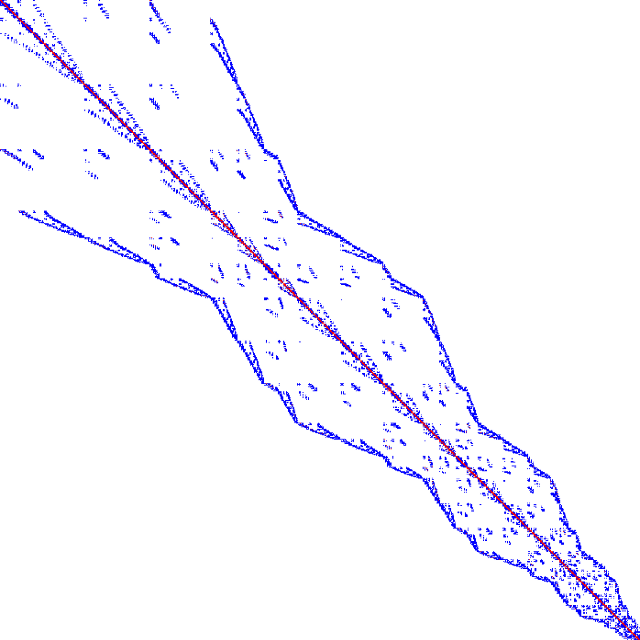
\includegraphics[width=.5\textwidth]{figures/EllipRCMSquare}
\end{center}
\end{frame}

\begin{frame}{Parallel Sparse Matrix}
\begin{itemize}
  \item Each process locally owns a submatrix of contiguous global rows
  \item Each submatrix consists of diagonal and off-diagonal parts
\end{itemize}

\begin{center}
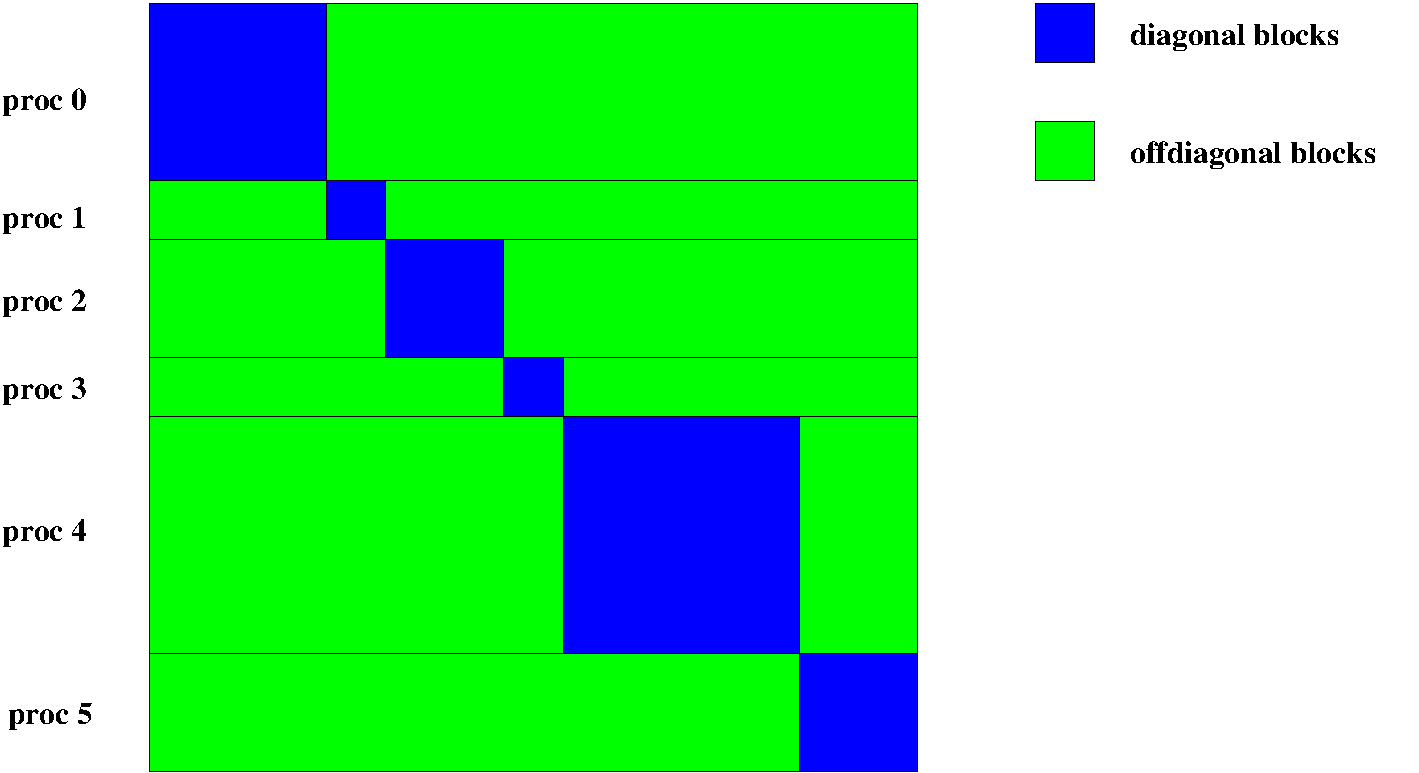
\includegraphics[width=3.5in]{figures/Mat/parallelSparseMatrix}
\end{center}

\begin{itemize}
  \item {\kb MatGetOwnershipRange(Mat A,int *start,int *end)}
  \begin{itemize}
    \item[{\kb start}:] first locally owned row of global matrix
    \item[{\kb end-1}:] last locally owned row of global matrix
  \end{itemize}
\end{itemize}
\end{frame}

\begin{frame}{Parallel Sparse Matrices}
\hbox{
\quad
\vbox{
{\kb MatMPIAIJSetPreallocation(Mat A, int dnz, int dnnz[], \\
  \qquad \qquad int onz, int onnz[])}
\begin{itemize}
  \item[dnz:] expected number of nonzeros in any row in the diagonal block
  \item[dnnz(i):] expected number of nonzeros in row i in the diagonal block
  \item[onz:] expected number of nonzeros in any row in the offdiagonal portion
  \item[onnz(i):] expected number of nonzeros in row i in the offdiagonal portion
\end{itemize}
}
}
\end{frame}

\begin{frame}{Verifying Preallocation}
\begin{itemize}
  \item Use runtime options \\
    {\kb -mat\_new\_nonzero\_location\_err} \\
    {\kb -mat\_new\_nonzero\_allocation\_err}
  \item Use runtime option {\kb -info}
  \item Output: \\
{\kb
  $[$proc \#$]$ Matrix size: \%d X \%d; storage space: \%d unneeded, \%d used \\
  $[$proc \#$]$ Number of mallocs during MatSetValues( )  is \%d
}
\end{itemize}

\bigskip

\begin{center}
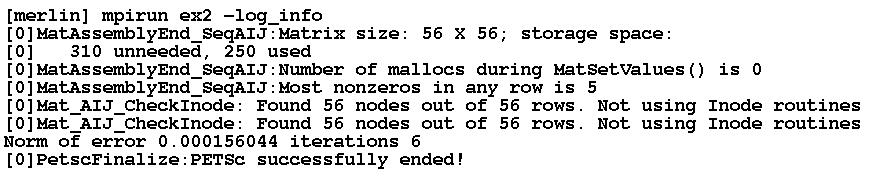
\includegraphics[width=5in]{figures/PETSc/logInfoOutput}
\end{center}
\end{frame}

\begin{frame}{Block and symmetric formats}
  \begin{itemize}
  \item BAIJ
    \begin{itemize}
    \item Like AIJ, but uses static block size
    \item Preallocation is like AIJ, but just one index per block
    \end{itemize}
  \item SBAIJ
    \begin{itemize}
    \item Only stores upper triangular part
    \item Preallocation needs number of nonzeros in upper triangular \\
      parts of on- and off-diagonal blocks
    \end{itemize}
  \item \code{MatSetValuesBlocked()}
    \begin{itemize}
    \item Better performance with blocked formats
    \item Also works with scalar formats, if \code{MatSetBlockSize()} was called
    \item Variants \code{MatSetValuesBlockedLocal()}, \code{MatSetValuesBlockedStencil()}
    \item Change matrix format at runtime, don't need to touch assembly code
    \end{itemize}
  \end{itemize}
\end{frame}

